\chapter[Os dados]{Os dados}

Neste capítulo será tratada as características dos dados disponíveis para este trabalho.

\section{Extração dos textos}

O STF disponibilizou os processos e suas peças no formato PDF. Nos arquivos recebidos, haviam volumes e peças já separadas.

Para obter o texto deste documentos, utilizou-se da ferramenta XpdfReader\footnote{Utilizou-se os comandos \textbf{pdftotext} e \textbf{pdftopng}. Disponível em: \url{https://www.xpdfreader.com/pdftotext-man.html}. Acesso em: 17-06-2018.} para extrair o texto das páginas de um PDF que estava em formato digital ou digitalizado com uma camada de texto.

Quando encontrada uma página sem texto, transformou-se esta em uma imagem para, em seguida, aplicar um reconhecedor ótico de caracteres (do inglês \textit{Optical Character Recognition} OCR).

\section{Tratamento dados}

Utilizou-se apenas parte dos dados para realizar a análise. Fez-se a limpeza utilizando expressões regulares \cite{GOYUAERTS2012} a fim de:

\begin{itemize}
	\item Remover caracteres especiais, tais como: \# @ $\backslash n$ 0xCE
    \item Remover números misturados com letras.
    \item Remover números
    \item Capturar leis, artigos e decretos.
    \item Remover espaços em branco
    \item Remover e-mail e \textit{link}.
\end{itemize}

Em seguida, aplicou-se as técnicas de radicalização, normalização \cite{SINGH2016} e remoção de palavras recorrentes \cite{MANNING2008}.

Além das palavras recorrentes, foram removidos nomes de pessoas e algumas palavras chaves específicas: 'elytho', 'neve', 'chenaud', 'tayrone', 'besen', 'youngéqyoung', 'sarubbi', 'balogh', 'pezarini', 'zezinho', 'intdo', 'izmailov', 'zotto', 'angelicoadvogados', 'limar', 'steiger', 'acidelma', 'vitoriar', 'tic', 'valcy', 'dadico', 'aloisia', 'itos', 'tendolo', 'rossol', 'catapani', 'cleudes', 'her', 'araçatuba', 'boeing', 'melar', 'rs', 'onaita', 'britar', 'ferreiro', 'licht', 'josé'.

Os nomes de pessoas coletados para adicionar na remoção de palavras, foram obtidos através da mineração dos dados abertos do governo\footnote{Arquivo da data de Janeiro/2017 dos gastos diretos. Disponível em: \url{http://www.portaldatransparencia.gov.br/downloads/mensal.asp?c=FavorecidosGastosDiretos}. Acesso em: 17-06-2018}, com o procedimento do Apêndice \ref{sec:apendiceA}. 

\section{Características dos dados}

Como abordado na Seção \ref{sec:problema}, os rótulos das peças já separadas advindas do STF não são confiáveis. Por conta disso, especialistas da área jurídica iniciaram o rotulamento adequado a estes documentos, classificando apenas em 7 categorias e Outros, apresentados na Tabela \ref{tab:categoriasPecas}.

A quantidade de documentos obtidos são apresentados na Tabela \ref{tab:categoriasPecas}. Nela, percebe-se que as peças de Agravo, Sentença, Petição de Agravo, Despacho de Agravo e Recurso Extraordinário estão com uma contagem não distribuída.

\begin{table}[h]
	\centering    
	\caption[Quantidade de cada peças]{Quantidade de cada peças. Fonte: elaboração própria.}
    \label{tab:categoriasPecas}
	\begin{tabular}{|l|c|c|}
    \hline
    \textbf{Tipo} & \textbf{Quantidade total} & \textbf{tamanho relativo} \\ 
    \hline
    Outro &  2.285 & $\times$ 142,81  \\
    \hline
    Agravo de Recurso Extraordinário & 1795 & $\times$  112,18  \\
    \hline
    Acordão & 1.568 & $\times$ 98,00  \\
    \hline
    Sentença & 252 & $\times$ 15,75  \\
    \hline
    Despacho & 89 & $\times$ 5,56  \\
    \hline
    Petição de Agravo & 63 & $\times$ 3,93  \\
    \hline
    Despacho de Agravo & 26 & $\times$ 1,62  \\
    \hline
    Recurso Extraordinário & 16 & $\times$ 1,00  \\
    \hline
    \textbf{Total} & 6094 & - \\
    \hline

    \end{tabular}
\end{table}

Após o tratamento dos dados, buscou-se por documentos com o mesmo conteúdo que tivessem classificações diferentes. Neste cenário, obteve-se 428 (7.00\%) documentos com confusão. As categorias que se confundiram foram as tuplas Outros e Acórdão, Agravo de Recurso Extraordinário e Recurso Extraordinário, Despacho e Outros, Acórdão e Sentença, e por último Petição de Agravo e Outros.

Como resultado do pre-processamento, obteve-se os resultados da Tabela \ref{tab:simbolos}, na qual transformou-se os textos em símbolos para realizar as contagens de símbolos.

\begin{table}[h]
	\centering    
	\caption[Métricas dos documentos]{Métricas dos documentos. Fonte: elaboração própria.}
    \label{tab:simbolos}
	\begin{tabular}{|l|c|}
    \hline
    \textbf{Nome} & \textbf{Valor} \\ 
    \hline
    Menor número de símbolos & 113 \\
    \hline
    Maior número de símbolos & 7.036 \\
    \hline
    Média de símbolos por documento & 1.113,17 \\
    \hline
    Total de símbolos & 6.783.709 \\
    \hline
    Tamanho do vocabulário & 20.009 \\
    \hline
    \end{tabular}
\end{table}

Antes de treinar um modelo classificador, fez-se uma correlação entre as classes com o BoW relativo ao total de cada palavra (Equação \ref{eq:bowRelativo}. Ou seja, o corpo de texto de cada tipo de documento foi concatenado, logo após, a contagem de palavras em cada tipo foi dividido pelo total de ocorrências em todos os documentos. Na Equação \ref{eq:bowRelativo}, o $i$ representa o tipo de documento e o $j$ representa a palavra pertencente ao dicionário.

\begin{equation}
\label{eq:bowRelativo}
	BoWrelative_{i,j} = \frac{BoW_{i,j}}{BoWt_{j}} \times 100
\end{equation}

A partir desse resultado, fez-se a correlação de spearman para gerar uma matriz triangular. Os valores para o coeficiente de spearman tem os intervalos entre $[-1,1]$. Os dados observados na Figura \ref{fig:correlacaoPecas} mostram que não há forte correlação entre os documentos, na qual o maior valor presente é a correlação inversa entre Outros e a peça ARE.

\begin{figure}[h]
  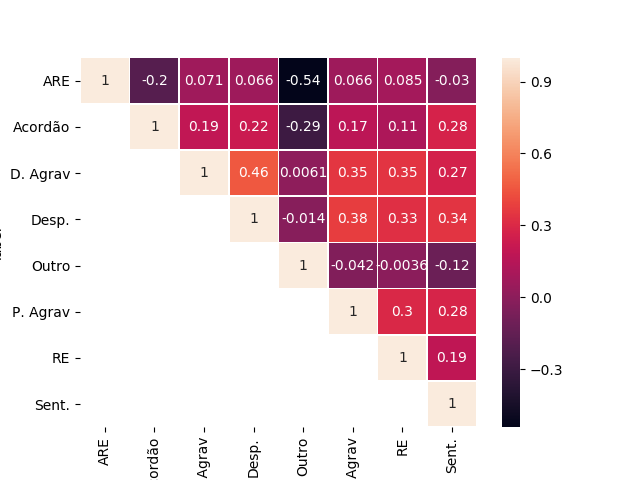
\includegraphics[keepaspectratio=true,scale=0.5]{figuras/correlacaoPecas}
  \centering
  \caption[Mapa de calor para correlação entre peças]{Mapa de calor para correlação entre peças. Fonte: GPAM \protect\footnotemark}
  \label{fig:correlacaoPecas}
\end{figure}
\footnotetext{O Grupo de Pesquisa em Aprendizado de Máquina (GPAM) está envolvido na tarefa de classificar peças para o STF. Esta imagem foi gerada para a exploração de dados realizada no projeto.}

Mesmo com a duplicação de rótulos nos documentos, utilizou-se a implementação do SVM Linear \cite{HEARST1995} para treinar com todos os dados, a fim de obter uma caracterização das palavras mais importantes. Os parâmetros utilizados foram os padrões de acordo com a implementação de \citeauthor{PEDREGOSA2011} (\citeyear{PEDREGOSA2011}), modificando apenas o número máximo de iterações para 50.000, pois somente com este valor que garantiu-se a convergência do modelo.

\begin{figure}[h]
	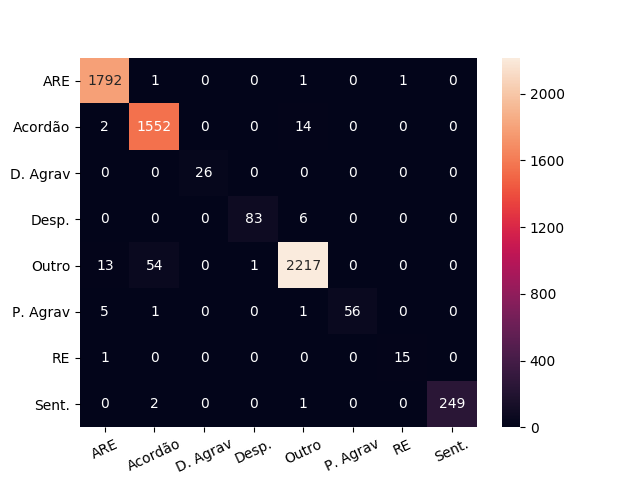
\includegraphics[keepaspectratio=true,scale=0.5]{figuras/confusionMatrixSMV}
    \centering
	\caption[Matriz de confusão para extração de características usando SVM]{Matriz de confusão para extração de características usando SVM. Fonte: elaboração própria}
	\label{fig:svmDisperssao}
\end{figure}

A figura \ref{fig:svmDisperssao} mostra que o modelo conseguiu separar bem as peças, e portanto, a Tabela \ref{tab:caracteristicasImportantes} mostra as características mais importantes extraídas dos vetores de suporte \cite{HEARST1995}.

Muitas palavras que não fazem sentido para o contexto do conteúdo das peças, como nomes próprios, apareceram de forma muito frequente durante a classificação (Exemplo: 'piauí', 'ubaldino', 'glacy', 'crisanto'). Apesar disso, as peças ARE, RE, Sentença e Despacho de Agravo mostraram palavras de importância significativas. Na tabela \ref{tab:caracteristicasImportantes}, as palavras relevantes de acordo com a Seção \ref{sec:cpc} estão em negrito.


\begin{table}[h]
  \centering
  \caption[Características importantes extraídas dos vetores de suporte]{Características importantes extraídas dos vetores de suporte. Fonte: Elaboração própria.}
  \label{tab:caracteristicasImportantes}
  \begin{tabular}{|p{1cm}|m{1.5cm}|m{1.5cm}|m{1.5cm}|m{1.5cm}|m{1.5cm}|m{1.5cm}|m{1.5cm}|m{1.5cm}|}
  	\hline
	\textbf{Pos} & \textbf{Agr. RE} & \textbf{Acórdão} & \textbf{D. Agr.} & \textbf{Desp.} & \textbf{Outro} & \textbf{P. Agr.} & \textbf{RE} & \textbf{Sen- \newline tença} \\ \hline
	1 &  https & liar & monsani & marmelo & ubaldino & sulmar & \textbf{artigo\newline\_102} & montrazi \\ \hline
	2 &  \textbf{extraor-\newline dinário} & chegar & munici- \newline pio & rollin & sumie & glacy & \textbf{consti-\newline tuição} & \textbf{inspeção} \\ \hline
    3 &  quintar & borrar & dezembro & amina- \newline dabe & minhos & bradesco & iii & \textbf{decidir} \\ \hline
    4 &  bandeiro & pg & município & cear & membro & \textbf{ag} & presentar & requis \\ \hline
    5 &  toste & piauí & vigência & spprev & crispin & vencedor & \textbf{venia} & \textbf{dispen- \newline sar} \\ \hline
    6 &  muci- \newline ciaria & filhar & obser- \newline vância & previ- \newline dencia & rizar & marcar & objeto & \textbf{artigo \newline \_42} \\ \hline
    7 &  unimed & \textbf{recurso} & \textbf{instru- \newline mentar} & líbero & parcial & \textbf{regi- \newline mental} & alínea & invalidez \\ \hline
    8 &  \textbf{federar} & carrá & blumenau & cásper & cleci & sortear & \textbf{reper- \newline cussão} & \textbf{funda- \newline mentar} \\ \hline
    9 &  acessar & unani- \newline midade & prever & itau & vanin & paraiba & incisar & moléstia \\ \hline
    10 &  quo & universo & termo & \textbf{recu- \newline perar} & ller & crisanto & dispositivo & expor \\ \hline
    11 & \textbf{juizado} & agostar & \textbf{lei \newline \_13256} & recupe- \newline ração & evori & ferrar & \textbf{recursal} & \textbf{postular} \\ \hline
    12 &  novembro & batistuzo & \textbf{regi- \newline mental} & creditos & pastar & incs & respeito & \textbf{produzir} \\ \hline
    13 &  diretoria & eichherr & assistir & fundação & especial & aguardar & presença & represen- \newline tante \\ \hline
    14 &  denega- \newline tório & dezembro & recursais & pintar & \textbf{agravo} & pf & \textbf{juizados} & julga- \newline mento \\ \hline
    15 &  trâmite & sangiogo & \textbf{presi- \newline dência} & represen- \newline tação & \textbf{artigo\newline \_48} & freuden- \newline thal & cabível & rocar \\ \hline
    16 &  segurar & autoprev & base & artigo\newline\_25 & suprir & obrigação & taubaté & íntegro \\ \hline
    17 &  eletroni- \newline camente & bitello & união & veiculos & \textbf{preâm- \newline bulo} & servidor & \textbf{razão} & capaci- \newline dade \\ \hline
    18 &  enviar & entre- \newline tanto & alterar & mjr & \textbf{cnj} & paraíba & exa & \textbf{código} \\ \hline
    19 &  \textbf{proces- \newline sual} & registrar & \textbf{lei\newline\_13105} & nelcis & paname- \newline ricano & efone & prolatado & intuito \\ \hline
    20 &  \textbf{artigo\newline\_544} & sedi- \newline mentar & repúblico & quantum & despachar & \textbf{previsto} & egrégio & procu- \newline rador \\ \hline
  \end{tabular}
\end{table}